\section{Results of simulations}\label{sec:results-of-simulations}
First, a baseline had to be found in which the system is more or less stable.
That is finding settings where almost no meals are discarded, and not many customers, and restaurants will leave.

Several automated runs were executed for one week ( 24 * 60 * 7 = 10.080 ticks) of simulation time.

The variables and default settings are:
\begin{center}
    \begin{tabular}{ |c|c|c| }
        \hline
        variables              & type & value \\
        \hline
        \hline
        number-of-restaurants & int & 10 \\
        \hline
        max-number-of-customers  & int & 500  \\
        \hline
        number-of-deliverers  & int & 15  \\
        \hline
        prepair\_time\_mean   & int & 15 \\
        \hline
        wait\_for\_deliverer  & int & 30 \\
        \hline
        deliverers\_may\_quit  & boolean & false  \\
        \hline
        radius\_allowed  & int & 64\\
        (max distance between &  &\\
        customer and restaurant)  & &\\
        \hline
    \end{tabular}
\end{center}

First, some runs with 15, 25 and 50 deliverers were executed.
This to find the effects of the number of delivers on the delivered (orange line) and discarded meals (green line).

The total number of orders is by the way correct, there are 500 customers, each customer on average orders once a week,
so around 500 orders in a week is expected.

The results from figures ~\ref{fig:examples 1 2 3} show that no big differences exists between 10, 25 and 50 deliverers.

\begin{center}
    \begin{figure*}
        \centering
        \begin{subfigure}[m]{0.30\textwidth}
            \centering
            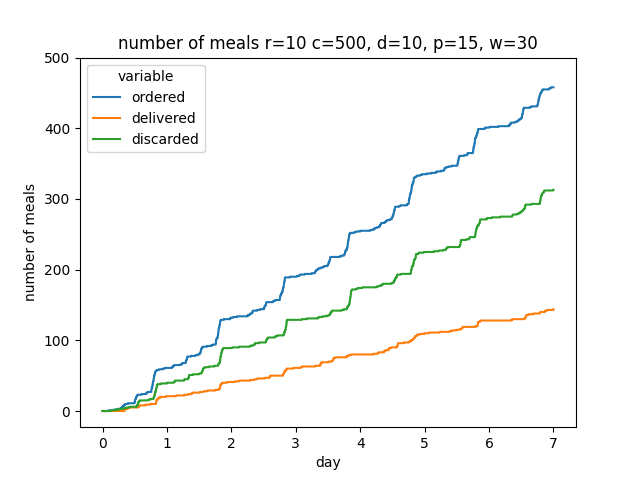
\includegraphics[width=\textwidth]{sections/run1/week_ed_food_ordering_distribution_500_10_10_30}
            \caption{example 1, 10 deliverers}
        \end{subfigure}
        \hfill
        \begin{subfigure}[m]{0.30\textwidth}
            \centering
            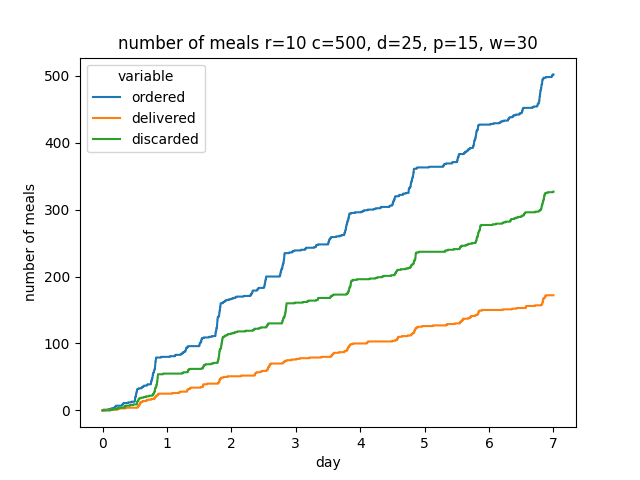
\includegraphics[width=\textwidth]{sections/run1/week_ed_food_ordering_distribution_500_10_25_30}
            \caption{example 2, 25 deliverers}
        \end{subfigure}
        \hfill
        \begin{subfigure}[m]{0.30\textwidth}
            \centering
            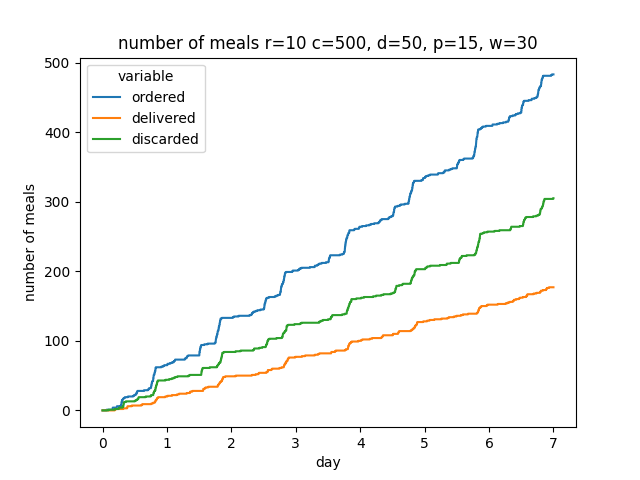
\includegraphics[width=\textwidth]{sections/run1/week_ed_food_ordering_distribution_500_10_50_30}
            \caption{example 3, 50 deliverers}
        \end{subfigure}
        \caption{Examples waiting time 30, radius 64 }
        \label{fig:examples 1 2 3}
    \end{figure*}
\end{center}

The reason for this is that the distances a driver has to make are too long, or the discarding waiting time is too short.
The deliverer has to drive towards the restaurant, and if it takes too long, the meal gets discarded.
Something has to be done about the other variables.

For the next set of runs, the wait times were set longer (60 minutes) and the radius allowed made shorter (32 patches).
This way drivers have more time to make it to the restaurant.
The distances between restaurants and customers are shorter because of the lower radius, thus deliverers are able to deliver faster and are sooner available for the next order.

The results are shown in figure~\ref{fig:examples 4 5 6}.

\begin{center}

    \begin{figure*}
        \centering
        \begin{subfigure}[m]{0.30\textwidth}
            \centering
            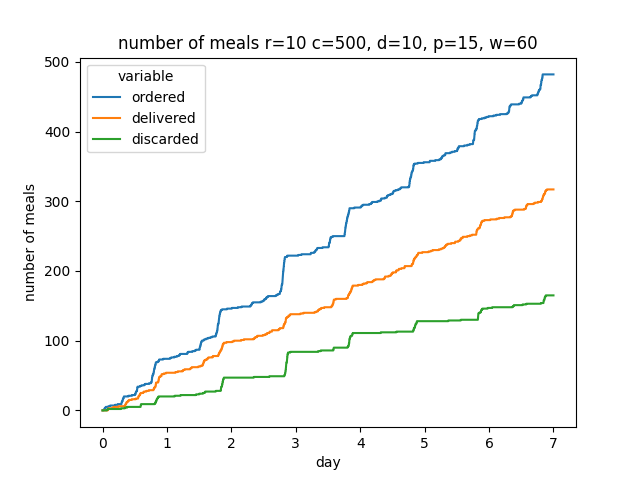
\includegraphics[width=\textwidth]{sections/run2/week_nm_rad_32food_ordering_distribution_500_10_10_60}
            \caption{example 4, 10 deliverers}
        \end{subfigure}
        \hfill
        \begin{subfigure}[m]{0.30\textwidth}
            \centering
            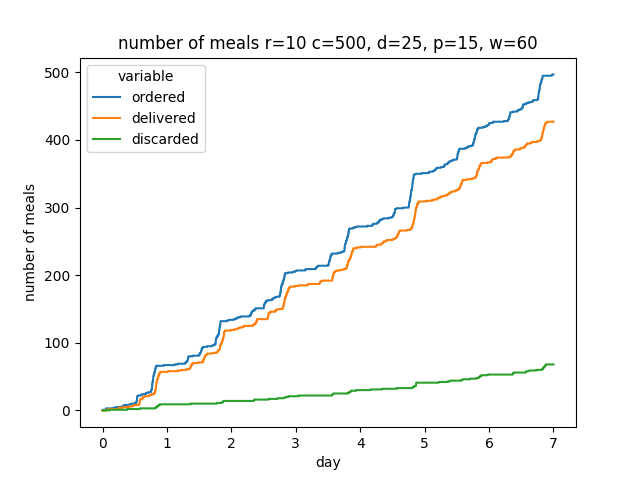
\includegraphics[width=\textwidth]{sections/run2/week_nm_rad_32food_ordering_distribution_500_10_25_60}
            \caption{example 5, 25 deliverers}
        \end{subfigure}
        \hfill
        \begin{subfigure}[m]{0.30\textwidth}
            \centering
            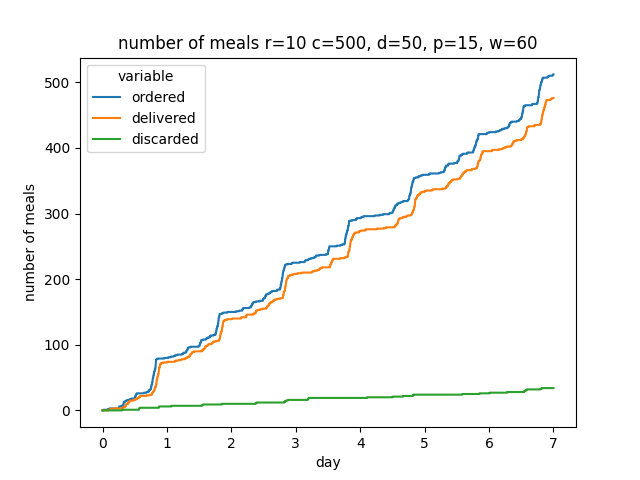
\includegraphics[width=\textwidth]{sections/run2/week_nm_rad_32food_ordering_distribution_500_10_50_60}
            \caption{example 6, 50 deliverers}
        \end{subfigure}
        \caption{Examples waiting time 60, radius 32 }
        \label{fig:examples 4 5 6}
    \end{figure*}
\end{center}

There is a difference now, many more of the meals are delivered.

To find out how many deliverers to hire, simulations where 3 times repeated with numbers of deliverers from 10 to 60.

The result of these simulations are depicted in  figure~\ref{fig:multiruns}.

\begin{figure*}
\centering
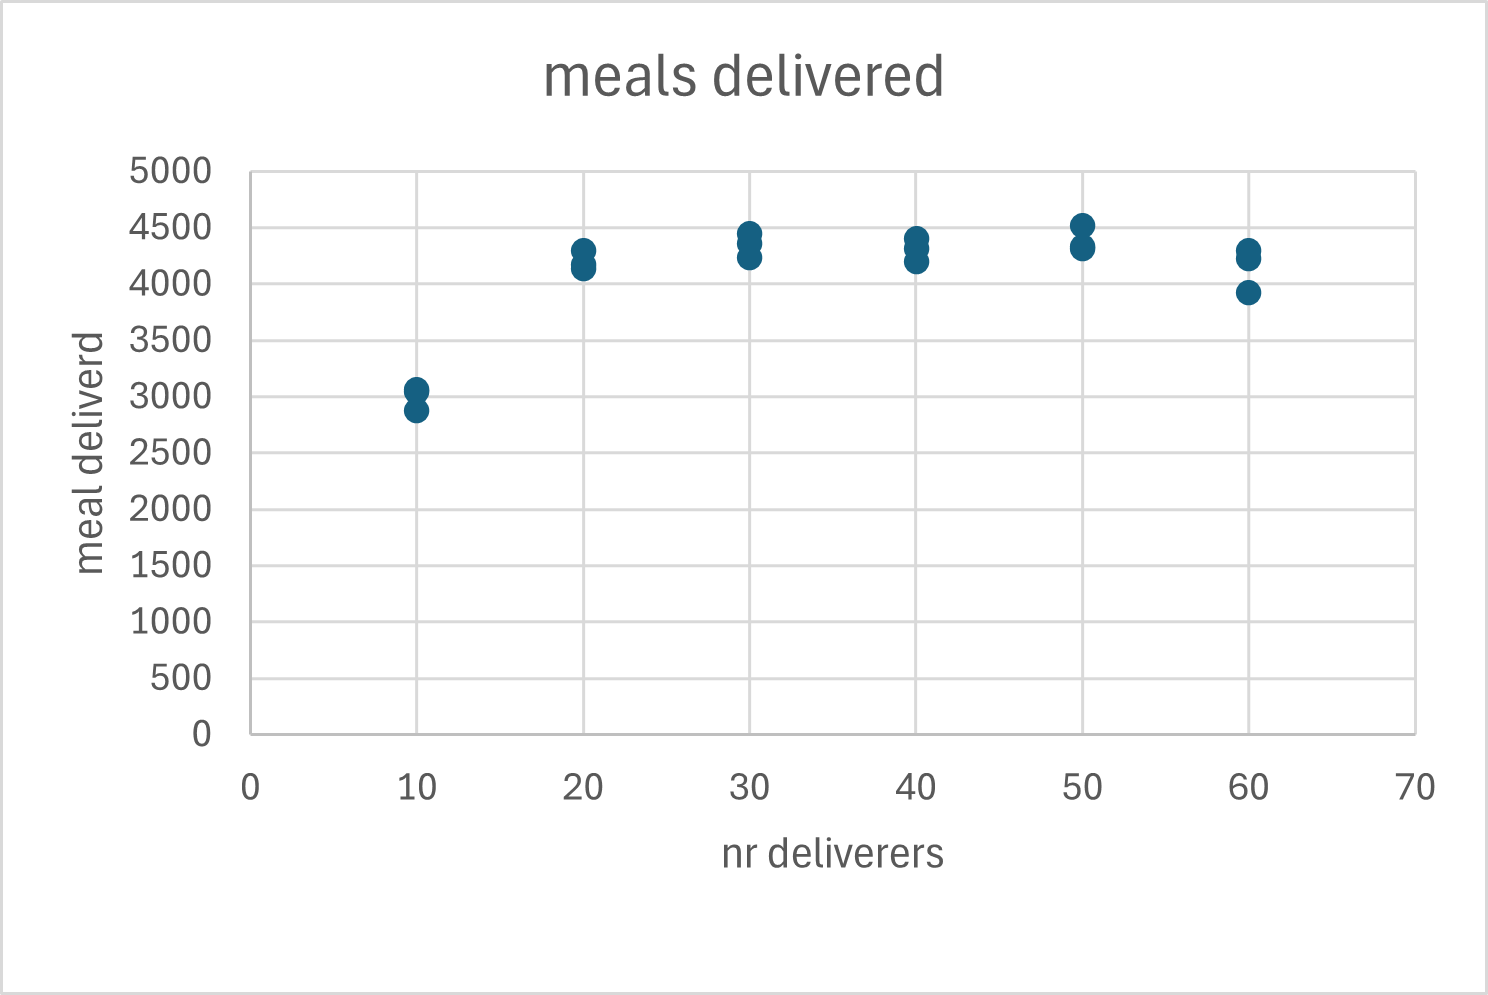
\includegraphics[width=12cm]{sections/pics/Afbeelding1}
\caption{meals delivered in 10 weeks, 3 runs per numbers of deliverers, waiting time 60 and radius 32 }
\label{fig:multiruns}
\end{figure*}

The numbers are the same with 20 deliverers or more.

With this information, the baseline is set.

The best result would be expected at a wait time of 60 minutes and 20 deliverers; more deliverers will not improve much.

\subsection{Model variant 1}\label{subsec:model-variant-1}
The baseline is determined with the next settings:
\begin{center}
    \begin{tabular}{ |c|c|c| }
        \hline
        variable              & type & default \\
        \hline
        \hline
        number-of-restaurants & int  & 10      \\
        \hline
        number-of-customers   & int  & 500     \\
        \hline
        number-of-deliverers  & int  & 20      \\
        \hline
        prepair\_time\_mean   & int  & 15      \\
        \hline
        wait\_for\_deliverer  & int  & 60      \\
        \hline
    \end{tabular}
\end{center}

On three runs of simulated ten weeks, the results are:

\begin{center}
    \begin{tabular}{ |c|c|c|c|c| }
        \hline
        meals & meals &  percentage  &  rest. & cust.  \\
        ordered & delivered & delivered &  left  & left \\
        \hline
        \hline
        4873          & 4292           & 0.88             & 9  & 488                \\
        \hline
        4916          & 4140           & 0.84             & 9  & 479               \\
        \hline
        4721          & 4176           & 0.88            & 9   & 475              \\
        \hline
        \hline
        4836          & 4202           & 0.86             & 9 & 480  \\
        \hline
    \end{tabular}
\end{center}

A deliverer delivers an average 4836/(20*10)= 24.18 meals per week.


\subsection{Model variant 2}\label{subsec:model-variant-2}
For the second variant, deliverers may leave if they don't make enough money; in this setting, only the number of deliveries is counted for simplicity.

In the previous section, a deliverer may have heard that a deliverer can deliver 24.18 per week.

In this variant, if a deliverer delivers less than this number, rounded to 24, in a week, they will stop delivering.
The delivery company knows it can deliver 4836 in 10 weeks and expects this also in this system.

The simulation is rerun for ten weeks.

The following table contains the results:
\begin{center}
    \begin{tabular}{ |c|c|c|c|c|c| }
        \hline
        meals   & meals     &  percentage  & del. &  rest. & cust. \\
        ordered & delivered & delivered    & left &  left  & left  \\
        \hline
        \hline
        4511          & 3483           & 0.77    & 11         & 8  & 429                \\
        \hline
        4557          & 3468           & 0.76    & 11         & 7  & 410               \\
        \hline
        4530          & 3667           & 0.80    & 12         & 8   & 446              \\
        \hline
        \hline
        4532          & 3539           & 0.78    & 11         & 8  & 428  \\
        \hline
    \end{tabular}
\end{center}

The number of deliverers has dropped 45\% but the number of delivered meals has dropped with 16\%

What is interesting is to see what the average number of meals delivered per deliverer is over the weeks; this is shown in figure~\ref{fig:average}.

\begin{figure*}
\centering
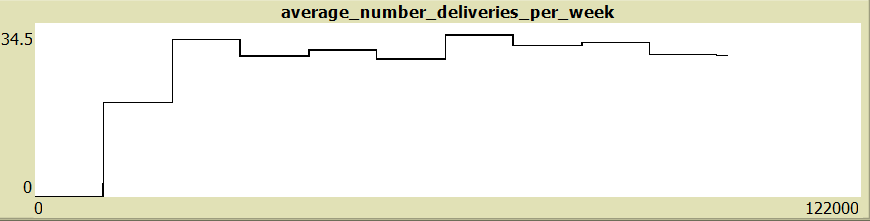
\includegraphics[width=12cm]{sections/pics/img}
\caption{NetLogo graph containing average deliveries per deliverer per week.}
\label{fig:average}
\end{figure*}

This graph shows that because many deliverers drop out in the beginning, the average for the remaining deliverers is higher compared to Model 1.

The result of this simulation is that giving deliverers a steady job will increase the number of meals delivered for the company.
However, the average per deliverer is lower than in a system where deliverers can decide to leave if the deliveries are less than those for a certain job.

Because more deliveries occur, the company could even pay them less per delivery and keep them onboard.

Of course, this is a highly abstract world, but it does say something about why delivery companies prefer the latter system.
It is also, on average, more profitable for the deliverers who remain, but not for the ones who left, of course.

\subsection{Conclusion}\label{subsec:conclusion}
A model has been created in NetLogo. It works as intended and reflects the delivery process in a very abstracted way.
Other researchers may use and adapt the model freely.

The simulations indicate that seeing the deliverers as independent contractors who stay when they earn enough is more advantageous to the companies and the deliverers.
But this says nothing about other factors like safety, sick leave, and working conditions.
More deliveries also mean more manual work; deliverers may get fatigued and risk their safety.

Luckily, in the real world, a combination exists: working for a lower solid income and getting a bonus for each delivery.






